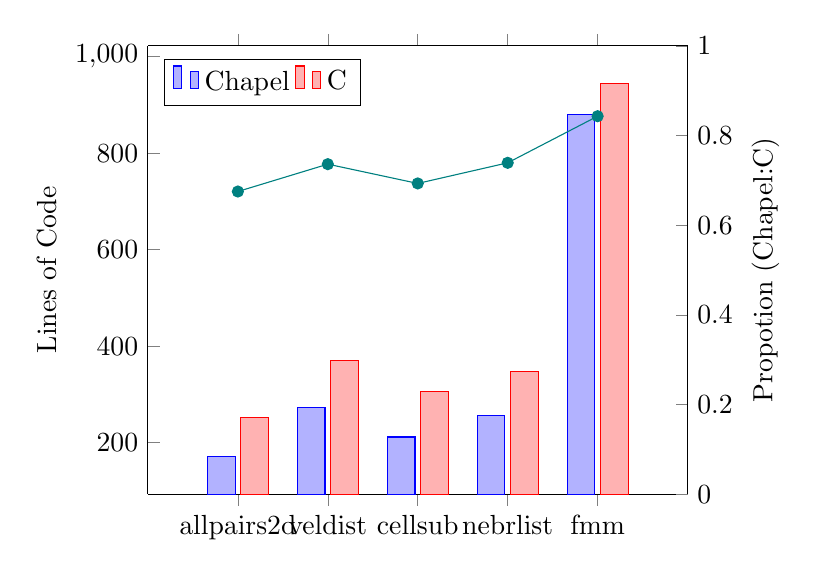
\begin{tikzpicture}
\begin{axis}[ybar, axis y line*=left,
  ylabel=Lines of Code, legend pos=north west, legend columns=2, xmin=0, xmax=6,
  xtick={1,2,3,4,5}, 
  xticklabels={allpairs2d, veldist, cellsub, nebrlist, fmm}]
\addplot plot coordinates
{(1, 171) (2, 273) (3, 212) (4, 257) (5, 880)};
\addplot plot coordinates
{(1, 253) (2, 371) (3, 306) (4, 348) (5, 945)};
\legend{Chapel, C}
\end{axis}

\begin{axis}[axis y line*=right,
  axis x line=none,
  ylabel=Propotion (Chapel:C),
  xmin=0, xmax=6, ymin=0, ymax=1]
\addplot[mark=*, color=teal] plot coordinates
{(1, 0.675) (2, 0.736) (3, 0.693) (4, 0.739) (5, 0.843)};
\end{axis}
\end{tikzpicture}
